\begin{exercise}
    It is sometimes necessary to convert a polynomial in BB form to monomial form.
    Consider a quadratic BB polynomial,
    \begin{equation*}
        p(x) = c_0 (1 - x)^2 + 2c_1 x(1 - x) + c_2 x^2.
    \end{equation*}
    Express $p$ in the monomial form
    \begin{equation*}
        p(x) = a_0 + a_1 x + a_2 x^2.
    \end{equation*}
\end{exercise}

\begin{solution}
    Rather than using the explicit formula for conversion, we can just expand the coefficients and collect terms.
    \begin{align*}
        p(x) &= c_0 (1 - x)^2 + 2c_1 x(1 - x) + c_2 x^2 \\
        &= c_0 (1 - 2x + x^2) + 2c_1 (x - x^2) + c_2 x^2 \\
        &= c_0 - 2c_0 x + c_0 x^2 + 2c_1 x - 2c_1 x^2 + c_2 x^2 \\
        &= c_0 + (-2c_0 + 2c_1) x + (c_0 - 2c_1 + c_2) x^2.
    \end{align*}
\end{solution}

\begin{exercise}
    Consider a polynomial $p(x)$ of degree $\leq d$, for arbitrary $d$.
    Show that if
    \begin{equation*}
        p(x) = \sum_{j=0}^d a_j x^j = \sum_{i=0}^d c_i B_i^d(x),
    \end{equation*}
    then
    \begin{equation*}
        a_j = \binom{d}{j} \Delta^j c_0.
    \end{equation*}
    \textit{Hint:} Use a Taylor approximation to $p$ to show that $a_j = p^{(j)}(0)/j!$. % chktex 40
\end{exercise}

\begin{solution}
    We have that
    \begin{equation*}
        p(x) = \sum_{j=0}^d a_j x^j = \sum_{i=0}^d c_i B_i^d(x).
    \end{equation*}
    By the Taylor approximation, we have that
    \begin{equation*}
        p(x) = p(x + 0) = \sum_{j=0}^d \frac{p^{(j)}(0)}{j!} x^j.
    \end{equation*}
    We thus have that
    \begin{equation*}
        a_j = \frac{p^{(j)}(0)}{j!}.
    \end{equation*}
    By properties of the Bézier curves, we have that
    \begin{equation*}
        p^{(j)}(x) = \frac{d!}{(d-j)!} \sum_{i = 0}^{d - j} \Delta^j c_i B_i^{d-j}(x),
    \end{equation*}
    and specifically for $x = 0$,
    \begin{equation*}
        p^{(j)}(0) = \frac{d!}{(d-j)!} \Delta^j c_0.
    \end{equation*}
    Combining these results, we have that
    \begin{equation*}
        a_j = \frac{p^{(j)}(0)}{j!} = \frac{d!}{(d-j)! j!} \Delta^j c_0 = \binom{d}{j} \Delta^j c_0,
    \end{equation*}
    as we wanted to show.
\end{solution}

\begin{exercise}
    We might also want to convert a polynomial from monomial form to BB form.
    Using Lemma 1.2, show that in the notation of the previous question,
    \begin{equation*}
        c_i = \frac{i!}{d!} \sum_{j=0}^i \frac{(d - j)!}{(i - j)!} a_j.
    \end{equation*}
\end{exercise}

\begin{solution}
    Lemma~1.2 states that for $j = 0, 1, \ldots, d$,
    \begin{equation*}
        x^j = \frac{(d - j)!}{d!} \sum_{i = j}^d \frac{i!}{(i - j)!} B_i^d(x).
    \end{equation*}

    We have that
    \begin{gather*}
        \sum_{j = 0}^d a_j x^j = \sum_{i = 0}^d c_i B_i^d(x) \\
        \sum_{j = 0}^d a_j \left[
            \frac{(d - j)!}{d!} \sum_{i = j}^d \frac{i!}{(i - j)!} B_i^d(x)
        \right]
        = \sum_{i = 0}^d c_i B_i^d(x) \\
    \end{gather*}
    As we have $i \geq j$, we can reorder the summation to the form $j \leq i$, by using
    \begin{equation*}
        \sum_{j = 0}^d \sum_{i = j}^d (\ldots) = \sum_{i = 0}^d \sum_{j = 0}^i (\ldots).
    \end{equation*}
    This gives us
    \begin{equation*}
        \sum_{i = 0}^d \left[
            \sum_{j = 0}^i a_j \frac{(d - j)!}{d!} \frac{i!}{(i - j)!}
        \right] B_i^d(x) = \sum_{i = 0}^d c_i B_i^d(x).
    \end{equation*}
    Which by isolating the coefficients, gives us
    \begin{equation*}
        c_i = \frac{i!}{d!} \sum_{j = 0}^i \frac{(d - j)!}{(i - j)!} a_j,
    \end{equation*}
    as we wanted to show.
\end{solution}

\begin{exercise}
    Implement the de Casteljau algorithm for cubic Bézier curves in Matlab or Python (or some other programming language), taking repeated convex combinations.
    Choose a sequence of four control points and plot both the control polygon and the Bézier curve, like those in Figure~1.3.
\end{exercise}

\begin{solution}
    The de Casteljau algorithm uses recursion to compute the value of a point along a Bézier curve by the following formula:
    \begin{enumerate}
        \item Initialize by setting $c_i^0 = c_i$ for $i = 0, 1, \ldots, d$.
        \item Then, for each $r = 1, 2, \ldots, d$, let
            \begin{equation*}
                c_i^r = (1 - x) c_i^{r-1} + x c_{i+1}^{r-1},
                \quad i = 0, 1, \ldots, d - r.
            \end{equation*}
        \item The last value $c_0^d$ is the value of the Bézier curve at $x$.
    \end{enumerate}

    This is implemented using Jax in Python in \verb|de_casteljau.py|, and the result is shown in Figure~\ref{fig:de_casteljau}, bearing a striking resemblance to the figure in the book.
    \begin{figure}[!ht]
        \centering
        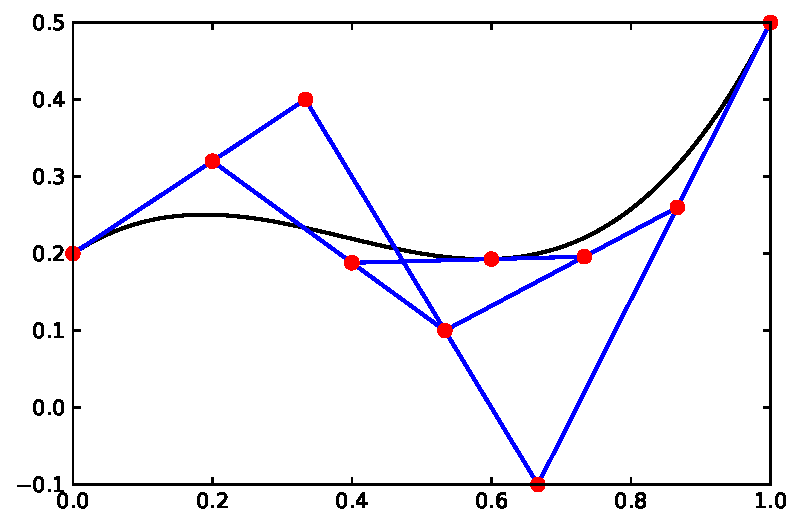
\includegraphics[width=0.6\textwidth]{1_bb_poly/de_casteljau.pdf}
        \caption{The de Casteljau algorithm applied to a cubic Bézier curve, with control points $(0.2, 0.4, -0.1, 0.5)$, illustrated at the point $x = 0.6$.\label{fig:de_casteljau}}
    \end{figure}
\end{solution}

\begin{exercise}
    Show that the graph, $g(x) = (x, p(x))$ of the BB polynomial $p$ in (1.6) is a Bézier curve in $\mathbb{R}^2$, with control points $(\xi_i, c_i)$, $i = 0, 1, \ldots, d$, where $\xi_i = i/d$.
    \textit{Hint:} Express $x$ as a linear combination of $B_0^d(x), \ldots, B_d^d(x)$.
\end{exercise}

\begin{solution}
    We can again utilize Lemma~1.2 to express $x$ as a linear combination of the Bernstein polynomials.
    We have that, writing $x = x^1$ for clarity,
    \begin{equation*}
        x^1 = \frac{(d - 1)!}{d!} \sum_{i = 1}^d \frac{i!}{(i - 1)!} B_i^d(x) = \sum_{i = 1}^d \frac{i}{d} B_i^d(x) = \sum_{i = 0}^d \frac{i}{d} B_i^d(x) = \sum_{i = 0}^d \xi_i B_i^d(x).
    \end{equation*}
    We can now express the graph of $p$ as a Bézier curve in $\mathbb{R}^2$ by
    \begin{equation*}
        g(x)
        = (x, p(x))
        = \left(
            \sum_{i = 0}^d \xi_i B_i^d(x), \sum_{i = 0}^d c_i B_i^d(x)
        \right)
        = \sum_{i = 0}^d (\xi_i, c_i) B_i^d(x)
        = \sum_{i = 0}^d \boldsymbol{c}_i B_i^d(x),
    \end{equation*}
    where $\boldsymbol{c}_i = (\xi_i, c_i)$ are the control points of the Bézier curve.
\end{solution}

\begin{exercise}
    Show that the tangent vector $\boldsymbol{p}'(x)$ of the Bézier curve in (1.6) lies in the convex cone of the vectors $\Delta \boldsymbol{c}_i$, i.e., in
    \begin{equation*}
        \text{cone}(\Delta \boldsymbol{c}_0, \ldots, \Delta \boldsymbol{c}_{d-1})
        = \left\{
            \sum_{i = 0}^{d-1} \mu_i \Delta \boldsymbol{c}_i
            : \mu_1, \ldots, \mu_{d-1} \geq 0
        \right\}.
    \end{equation*}
\end{exercise}

\begin{solution}
    The derivative (or perhaps \textit{gradient} is the correct term) of the Bézier curve $\boldsymbol{p}(x)$ is given by
    \begin{equation*}
        \boldsymbol{p}'(x)
        = d \sum_{i = 0}^{d-1} \left(
            \boldsymbol{c}_{i+1} - \boldsymbol{c}_i
        \right) B_i^{d-1}(x)
        = d \sum_{i = 0}^{d-1} \Delta \boldsymbol{c}_i B_i^{d-1}(x).
    \end{equation*}
    As $B_i^{d-1}(x) \geq 0$ for $x \in [0, 1]$, we can set $\mu_i = d B_i^{d-1}(x)$, and we have that
    \begin{equation*}
        \boldsymbol{p}'(x) = \sum_{i = 0}^{d-1} \mu_i \Delta \boldsymbol{c}_i \in \text{cone}(\Delta \boldsymbol{c}_0, \ldots, \Delta \boldsymbol{c}_{d-1}),
    \end{equation*}
    as we wanted to show.
\end{solution}

\begin{exercise}
    Show that the first derivative of $p$ in~(1.6) can be expressed (and computed) as
    \begin{equation*}
        p'(x) = d(c_{1}^{d-1} - c_{0}^{d-1}),
    \end{equation*}
    where $c_{1}^{d-1}, c_{0}^{d-1}$ are the points of order $d-1$ in de Casteljau's algorithm~(1.10).
\end{exercise}

\begin{solution}
    We have that
    \begin{equation*}
        p(x) = c_0^d = (1 - x) c_0^{d-1} + x c_1^{d-1},
    \end{equation*}
    and thus by differentiating with respect to $x$, we have that
    \begin{equation*}
        p'(x) = c_1^{d-1} - c_0^{d-1}.
    \end{equation*}
    This tells us that we cannot be as naive as this, as $c_0^d$ is actually a function of $x$, and not simply a constant.

    What we might instead need to note is that
    \begin{equation*}
        c_i^r = \sum_{j = 0}^r c_{i+j} B_j^r(x),
    \end{equation*}
    and combining this with the fact that
    \begin{equation*}
        \left( B_i^d \right)'(x) = d \left( B_{i-1}^{d-1} - B_i^{d-1} \right)(x),
    \end{equation*}
    we have that
    \begin{align*}
        p'(x)
        &= d \sum_{i = 0}^{d-1} \left( c_{i+1} - c_i \right) B_i^{d-1}(x)
        = d \left[
            \sum_{i = 0}^{d-1} c_{i+1} B_i^{d-1}(x) - \sum_{i = 0}^{d-1} c_i B_i^{d-1}(x)
        \right] \\
        &= d(c_{1}^{d-1} - c_{0}^{d-1}),
    \end{align*}
    as we wanted to show.
\end{solution}
